\documentclass{beamer}

% Theme
\usetheme{PaloAlto} % You can choose from various built-in themes

% Color theme (optional)
\usecolortheme{default} % You can choose from various built-in color themes

% Title page
\title{Alternating Series and Conditional Convergence}
\author{Avinash Iyer}
\institute{Occidental College}
\date{\today} % You can set a specific date here

% Additional packages (you can add more as needed)
\usepackage{graphicx} % For including images
\usepackage{caption}  % For customizing captions
\usepackage{amsmath}  % For mathematical symbols and equations
\usepackage{hyperref} % For hyperlinks

% Define custom colors (optional)
\definecolor{myblue}{RGB}{0,51,102}
\definecolor{myred}{RGB}{204,0,0}
\makeatletter
\renewrobustcmd{\beamer@@pause}[1][]{%
  \unless\ifmeasuring@%
  \ifblank{#1}%
    {\stepcounter{beamerpauses}}%
    {\setcounter{beamerpauses}{#1}}%
  \onslide<\value{beamerpauses}->\relax%
  \fi%
}
\makeatother
% Custom settings (optional)
\setbeamercolor{structure}{fg=myblue} % Change the color of the presentation elements
\setbeamertemplate{caption}[numbered] % Number captions for figures and tables
\AtBeginSection[]
{
  \begin{frame}
    \frametitle{Contents}
    \tableofcontents[currentsection]
  \end{frame}
}
\begin{document}

\begin{frame}
    \titlepage
\end{frame}
\begin{frame}
  \frametitle{Table of Contents}
  \tableofcontents
\end{frame}
\section{Alternating Harmonic Series: An Analysis}
\begin{frame}
  \frametitle{A Series}
  Consider the following series: \pause
  \begin{align*}
    \sum_{n=1}^{\infty} \frac{(-1)^{n + 1}}{n} \pause &= 1 \pause - \frac{1}{2} \pause + \frac{1}{3}\pause - \frac{1}{4} \pause + \frac{1}{5} - \cdots
  \end{align*} \pause
  This series appears to be related to the harmonic series, but also very different:
  \begin{align*}
    \sum_{n=1}^{\infty}\frac{1}{n} &= 1 + \frac{1}{2} + \frac{1}{3} + \frac{1}{4} + \cdots \tag*{Harmonic Series}
  \end{align*}
\end{frame}
\begin{frame}
  \frametitle{Divergence of the Harmonic Series}
  We can show that the harmonic series is divergent using the series comparison test:
  \begin{align*}
    \sum_{n=1}^{\infty}\frac{1}{n} &= 1 + \frac{1}{2} + \frac{1}{3} + \frac{1}{4} + \frac{1}{5} + \cdots\pause\\
                                   &\geq 1 + \frac{1}{2} + \frac{1}{4} + \frac{1}{4} + \frac{1}{8} + \cdots\pause\\
                                   &= 1 + \frac{1}{2} + \frac{1}{2} + \frac{1}{2} + \cdots\pause\\
                                   &= \infty
  \end{align*}
\end{frame}
\begin{frame}
  \frametitle{Differences}
  However, our alternating harmonic series is different. Let's look at partial sums. \pause
  \begin{align*}
    s_{n} &= \sum_{k=1}^{n} \frac{(-1)^{n+1}}{n}\pause\\
    s_{1} &= 1\pause\\
    s_{2} &= \frac{1}{2}\pause\\
    s_{3} &= \frac{5}{6}\pause\\
    s_{4} &= \frac{7}{12}\\
          &\vdots
  \end{align*}
\end{frame}
\begin{frame}
  Clearly, this sequence does not grow without bound --- it is bounded above by $1$, and doesn't seem to dip below $\frac{1}{2}$.
  \begin{center}
    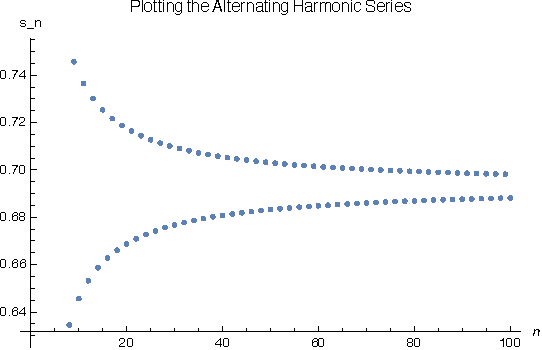
\includegraphics[width=0.8\textwidth]{images/alternating_harmonic_series_plot.pdf}
  \end{center}
\end{frame}
\begin{frame}
  \frametitle{Convergence}
  The alternating harmonic does converge. Courtesy of Wolfram MathWorld, we know that the series converges to the following:
  \begin{align*}
    \sum_{n=1}^{\infty}\frac{(-1)^{n+1}}{n} &= \ln 2
  \end{align*}\pause
  ...or does it? 
\end{frame}
\begin{frame}
  \frametitle{Rearranging the Alternating Harmonic Series}
  Rearrange the series as follows:
  \begin{align*}
    1 - \frac{1}{2} + \frac{1}{3} - \frac{1}{4} + \cdots &= \left(1-\frac{1}{2}\right) - \frac{1}{4} + \left(\frac{1}{3} - \frac{1}{6}\right) - \frac{1}{8} + \cdots\pause\\
                                                                       &= \frac{1}{2} - \frac{1}{4} + \frac{1}{6} - \frac{1}{8} + \cdots\pause\\
                                                                       &= \frac{1}{2}\sum_{n=1}^{\infty}\frac{(-1)^{n+1}}{n}\\
                                                                       &= \frac{1}{2}\ln 2
  \end{align*}
\end{frame}
\section{Conditional Convergence}
\begin{frame}
  \frametitle{Introduction to Conditional Convergence}
  \begin{itemize}
    \item<1-> We saw that our alternating harmonic series converges to $\ln 2$, but should it not converge to $\ln 2$ all the time?
    \item<2-> For example, no matter how we arrange
      \begin{align*}
        \sum_{n=0}^{\infty}\frac{1}{2^n},
      \end{align*}
      The sum should always equal $1$.
    \item<3-> Maybe we should redefine convergence?
  \end{itemize}
\end{frame}
\begin{frame}
  \frametitle{Alternating Series}
  \begin{itemize}
    \item<1-> The answer is that the alternating harmonic series is \textit{conditionally} convergent.
    \item<2-> We can always rearrange the terms of the alternating harmonic series to form whatever sum we want.
    \item<3-> In general, alternating series, of the form
      \begin{align*}
        \sum_{n=1}^{\infty}(-1)^{n+1}a_n
      \end{align*}
      can be convergent, while at the same time
      \begin{align*}
        \sum_{n=1}^{\infty} a_n
      \end{align*}
      is divergent.
  \end{itemize}
\end{frame}
\begin{frame}
  \frametitle{Alternating Series Test}
  \begin{itemize}
    \item<1-> In general, we can find if an alternating series is \textit{conditionally} convergent as follows:
    \begin{itemize}
      \item<2-> The (absolute value) series terms are strictly positive and decreasing.
        \begin{align*}
          0 < a_{n+1} < a_n
        \end{align*}
      \item<3-> The series terms tend to zero:
        \begin{align*}
          \lim_{n\rightarrow\infty}a_n = 0
        \end{align*}
    \end{itemize}
  \end{itemize}
\end{frame}
\begin{frame}
  \frametitle{Applying the Alternating Series Test}
   In the alternating harmonic series, we see that\pause
      \begin{align*}
        0 < \frac{1}{n+1} < \frac{1}{n},
      \end{align*}\pause
      and
      \begin{align*}
        \lim_{n\rightarrow\infty}\frac{1}{n} = 0.
      \end{align*} \pause
      So the series is \textit{conditionally} convergent.
\end{frame}
\section{Absolute Convergence}
\begin{frame}
  \frametitle{What is Absolute Convergence?}
  We know two facts: \pause
  \begin{itemize}
    \item<1-> The alternating harmonic series converges conditionally
    \item<2-> The harmonic series diverges
  \end{itemize}\pause
  We need a stronger term for series convergence --- \textit{absolute} convergence --- when a series converges to a single value.
\end{frame}
\begin{frame}
  \frametitle{Finding Absolute Convergence}
  If the absolute value of the terms in the series converges, then the series converges absolutely.\pause\\
  \begin{exampleblock}{Absolutely Convergent Alternating Series}
    \begin{align*}
      \sum_{n=0}^{\infty}\frac{(-1)^{n}}{2^n}
    \end{align*}
    converges absolutely. Why?\pause\\

    By the geometric series,
    \begin{align*}
      \sum_{n=0}^{\infty}\left|\frac{(-1)^{n}}{2^n}\right| = \sum_{n=0}^{\infty}\frac{1}{2^n}
    \end{align*}
    converges.
  \end{exampleblock}
\end{frame}
\section{Recap}
\begin{frame}
  \frametitle{What We Have Learned}
  \begin{itemize}
    \item<1-> The same series can converge to different values depending on the arrangement of terms --- known as \textit{conditional convergence}
    \item<2-> We can use the \textit{alternating series test} to find if a series converges conditionally.
    \item<3-> However, we would need to use other tools to find if a series is absolutely convergent.
  \end{itemize}
\end{frame}
\begin{frame}
  \frametitle{Questions?}
  Thank you for listening. Any questions?
\end{frame}
\end{document}
